%%%%%%%%%%%%%%%%%%%%%%%%%%%%%%%%%%%%%%%%%%%%%%%%%%%%%%%%%%%%%%%
%
% Introduction.tex (part of thesis.tex)
% author: Qie Hu
%
%%%%%%%%%%%%%%%%%%%%%%%%%%%%%%%%%%%%%%%%%%%%%%%%%%%%%%%%%%%%%%%

%!TEX root = ../../thesis.tex

\section{Problem Statement}
\label{sec:problem_statement}


%%%%%%%%%%%%%%%%%%%%%%%%%%%%%%%%%%%%%%%
\subsection{PJM Regulation Market Operation \normalfont{\cite{PJM11}}}

%PJM's reserve scheduling includes the day-ahead market and the hourly scheduling process.
In this section, we briefly describe the operation of the PJM regulation market relevant to this work, which involves the day-ahead market and the hourly scheduling process.
First, resources that wish to participate in the regulation market can submit their bids, which includes capacities and offering prices, one day ahead in the day-ahead market for the entire 24 hours of the operating day. 
%The regulation offer includes the regulation capability offer cost and the regulation performance cost of the resource.
After the day-ahead market closes, PJM calculates the initial regulation schedule for each hour of the operating day, based on bids, offers, submitted schedules and predicted reserve needs. %, amongst other requirements.
The hourly scheduling process operates at an overlapping time frame, and allows participating resources to declare their regulation capacities and baseline consumptions, which must remain fixed for each operating hour, up to 60 minute before the beginning of the operating hour.
\begin{assumption}
In this work, we assume that our building participates in the hourly reserve scheduling process.
\end{assumption}
%To participate in the regulation market, a demand resource must meet the following criteria. First, it must provide at least 0.1MW of regulation capacity. Second, 

During real time operation, a frequency regulation signal is sent from PJM to each participating resource every 2 seconds. In turn, the resource is required to regulate its instantaneous electricity consumption around its baseline such that the deviation tracks the regulation signal.

%In this work, we assume that an aggregation of buildings cooperate to participate in the regulation market. The regulation 


%%%%%%%%%%%%%%%%%%%%%%%%%%%%%%%%%%%%%%%

%\subsubsection{Building Description}\label{sec:building_description}
%The field experiments are conducted on the fourth floor of Sutardja Dai Hall (SDH), a seven-floor-building equipped with a VAV HVAC system on the University of California, Berkeley campus. 

%Inside the air handling unit (AHU), large supply fans drive air through heat exchangers, cooling it down to a desired supply air temperature (SAT). The cooled air is then distributed to VAV boxes located throughout the building. The flow rate and the final temperature of the supply air delivered to each room is then controlled by adjusting the damper position and the amount of reheating performed at the VAV boxes. 
%
%The fourth floor has a total area of 1300 square-meters and contains a variety of spaces such as individual offices, open workspaces, staircases and electrical rooms. 
%We divide the floor into six zones for modeling and control purposes (Figure \ref{fig:floor_plan}).

%\begin{figure}[h]
%\centering
%\vspace*{-0.4cm}
%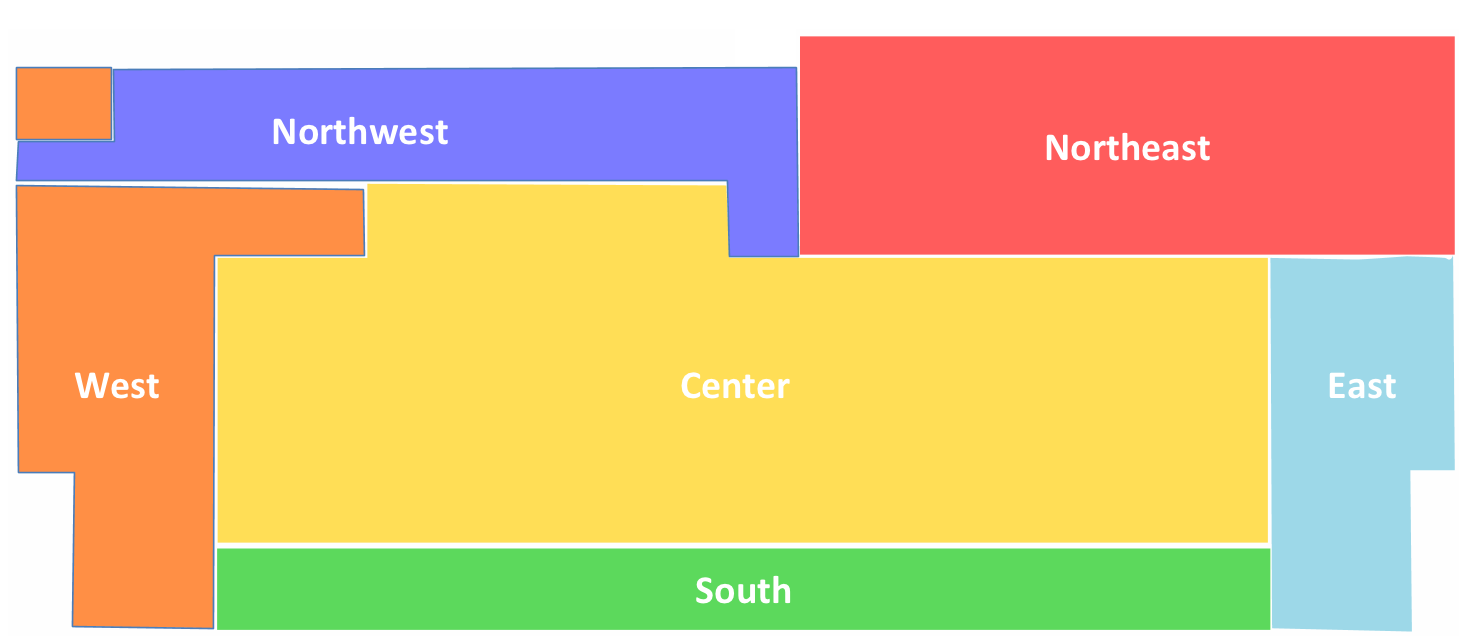
\includegraphics[scale=0.30]{chapters/building_exp/figures/FloorPlan.png}
%\vspace*{-0.05cm}
%\caption{Zones for the fourth floor of Sutardja Dai Hall.}
%\label{fig:floor_plan}
%\vspace*{-0.45cm}
%\end{figure}


%%%%%%%%%%%%%%%%%%%%%%%%%%%%%%%%%%%%%%%

\subsection{Control Scheme}\label{sec:control_scheme}
The field experiments are conducted on the fourth floor of SDH, i.e., the same building used for model identification in Chapter \ref{chapter:building_model}, which is a seven-floor-building equipped with a VAV HVAC system.
On the control system side, SDH is equipped with the Siemens' APOGEE system -- a BAS that controls the building's HVAC system and lighting based on existing control loops. %and 
The communication between the building automation devices is enabled by a building automation and control network (BACnet). 
We develop an external frequency regulation controller to read measurements from and send control commands to the HVAC equipment via the BACnet. 

Our goal is to adjust the instantaneous power consumption of the supply fans to provide frequency regulation while maintaining the indoor temperature on the fourth floor within the comfort zone.
We propose to control the supply fans' power consumption by adjusting their speed and use the airflow rates to the fourth floor for the comfort goal.
The airflow rates to the rooms are chosen not to depend on the frequency regulation signal because they have very different reaction times: the regulation signal is updated every 2 seconds, however the dampers in the VAV boxes have a  time constant in the order of minutes.
Consequently, our controller overrides the BAS' supply fans' speed control loops and the airflow rate control loops at the VAV boxes situated on the fourth floor. 
All other BAS' control loops are left intact.
Our proposed control architecture consists of a High Level Controller and a Low Level Controller as depicted in Figure \ref{fig:control_scheme}:

\begin{itemize}
	\item{High Level Controller (HLC) - Reserve Scheduling and Room Temperature Control}\label{sec:high_level}

A closed-loop Model Predictive Controller (MPC) that operates every hour. Its objective is two-fold: first, determine the reserve capacity that the building can reliably offer for the next operating hour; second, calculate the baseline airflow rate to each room that ensures occupant comfort while providing this amount of reserves.
Both the capacity and the baseline are chosen to minimize electricity cost and maximize rewards from reserve provision.

	\item{Low Level Controller (LLC) - Frequency Tracking}\label{sec:low_level}

A switched controller that modulates the speed of the supply fan every 4 seconds so that its power consumption deviations from its baseline tracks the frequency regulation signal.
It consists of a model-based feedforward controller and a Proportional Integral (PI) feedback controller.
As explained in Section \ref{sec:llc}, our switched controller has a different switching condition from \cite{Vrettos:2016flexlab1}, which makes our controller suitable for scenarios where the building is subject to larger disturbances.
\\
\\
Note that although PJM's regulation signal is updated every 2 seconds, power consumption measurements of the supply fans in SDH are only available every 10-20 seconds, therefore the LLC was chosen to run at an intermediate rate of 4 seconds. This is a restriction of our particular building. Using another building whose supply fans' power measurements are updated more frequently would only improve our controller's tracking performance.
\end{itemize}


\begin{figure}[t]
\centering
%\vspace*{-0.4cm}
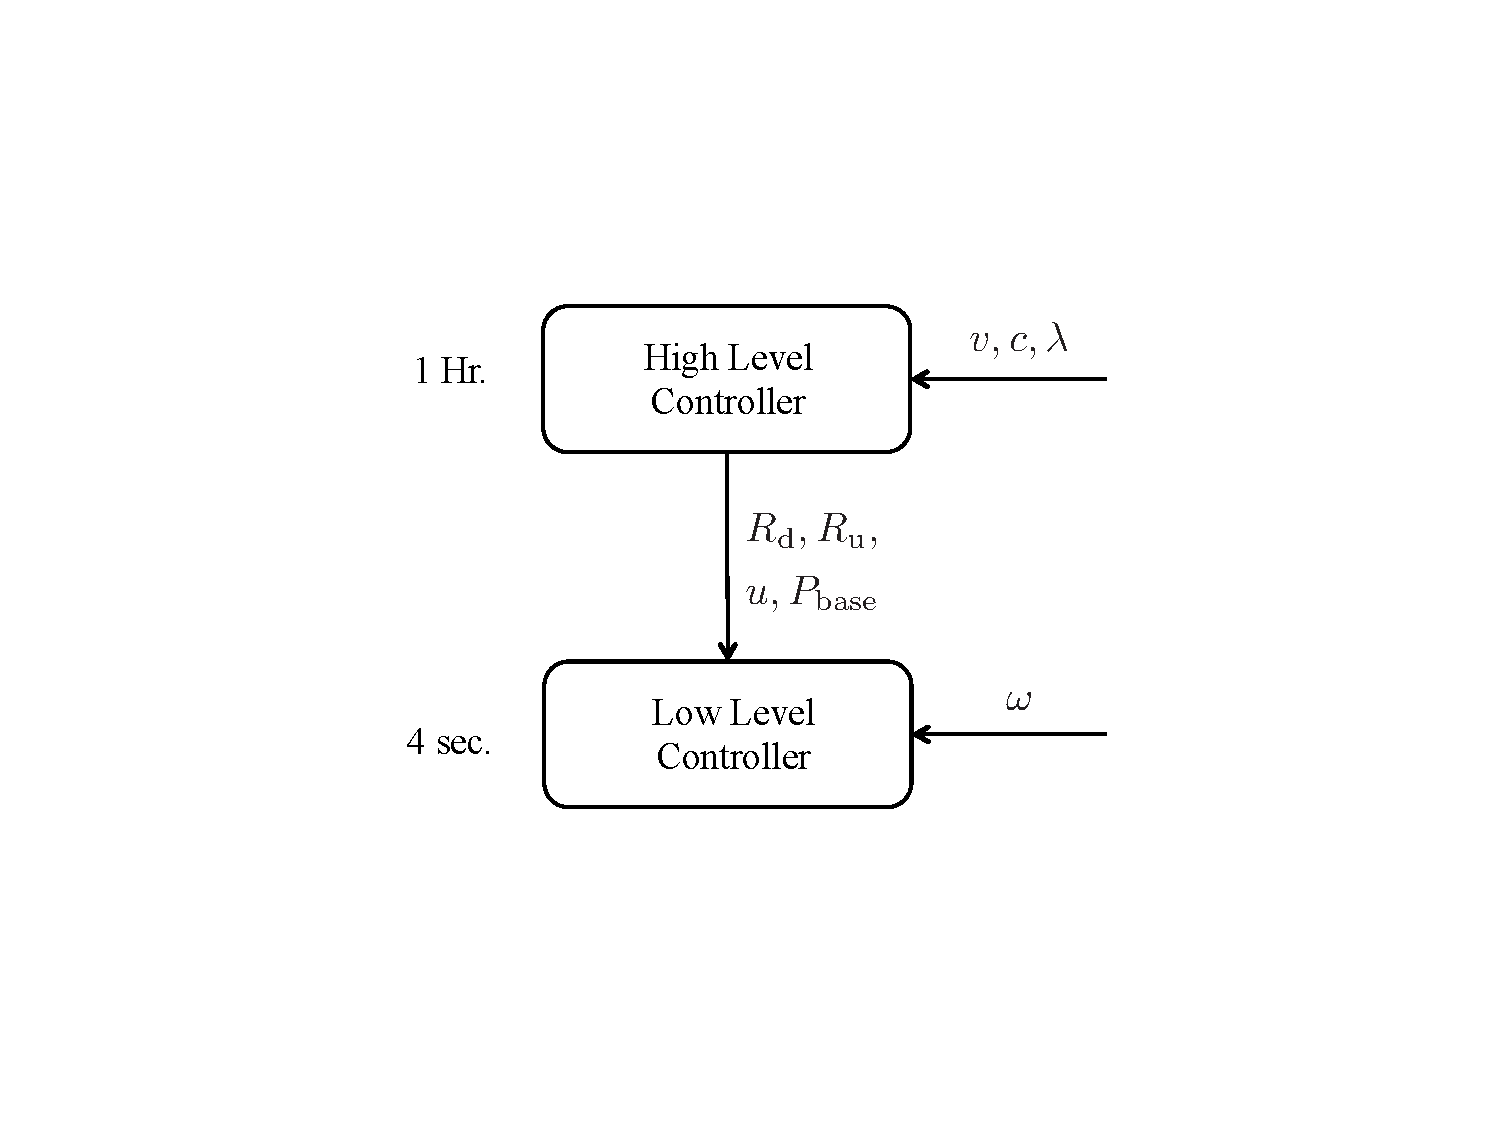
\includegraphics[scale=0.7]{chapters/building_exp/figures/control_scheme.pdf}
\vspace*{-0.05cm}
\caption{Two level control scheme for frequency regulation. See Table \ref{tab:notation} for description of symbols.}
\label{fig:control_scheme}
\vspace*{1cm}
\end{figure}

\begin{table}[b]
\centering
\caption{Table of notation.}
\label{tab:notation}
\begin{tabular}{ll}
\toprule
Symbol & Description \\ \hline
$R_{\text{u}}, R_{\text{d}}$ & Up- and down-regulation capacities \\
$P_{\text{base}}, P$ & Baseline and actual fan power consumption\\
$N_{\text{base}}, N$ & Baseline and actual fan speed\\
$x$ & Zone temperature\\
$u$ & Control input\\
$v$ & Disturbance\\%: ambient air temp., supply air temp.\\
$q$ & Internal gains\\
$w$ & Normalized frequency regulation signal\\
$c$ & Unit electricity cost\\
$\lambda$ & Reward for reserve provision\\
\bottomrule
\end{tabular}
\end{table}


%
%\begin{table}[b]
%\centering
%\begin{tabular}{ll}
%\toprule
%Symbol & Description \\ \hline
%$R_{\text{u},k}, R_{\text{d},k}$ & Up- and down-regulation capacities \\
%$P_{\text{base},k}, P_k$ & Baseline and actual fan power consumption\\
%$N_{\text{base},k}, N_k$ & Baseline and actual fan speed\\
%$x_k$ & Zone temperature\\
%$u_k$ & Control input\\
%$v_k$ & Disturbance\\
%$q_k$ & Internal gains\\
%$w_k$ & Normalized frequency regulation signal\\
%$c_k$ & Unit electricity cost\\
%$\lambda_k$ & Reward for reserve provision\\
%\bottomrule
%\end{tabular}
%\caption{Table of notation.}
%\label{tab:notation}
%\end{table}








